\documentclass[15pt]{extarticle}
\usepackage{graphicx}
\usepackage[utf8]{inputenc}
\usepackage[T1]{fontenc}
\usepackage{natbib}
\usepackage{lmodern}
\usepackage{titlesec}
\usepackage{tabularx}
\usepackage{gensymb}


\titlespacing*{\section}
{0pt}{10.0ex plus 1ex minus .2ex}{2.0ex plus .1ex minus .1ex}
\titlespacing*{\subsection}
{0pt}{6.0ex plus 1ex minus .2ex}{1.0ex plus .1ex minus .1ex}

% For enumerations with section number.
%\usepackage{enumitem}
%\setenumerate[1]{label=\thesection.\arabic*.}
%\setenumerate[2]{label*=\arabic*.}


\renewcommand{\familydefault}{\sfdefault}

\usepackage{geometry}
 \geometry{
 a4paper,
 left=20mm,
 right=20mm,
 top=20mm,
 bottom=30mm,
 }

\usepackage[colorlinks = true,
            linkcolor = blue,
            urlcolor  = blue,
            citecolor = black,
            anchorcolor = blue]{hyperref}

\setlength{\parskip}{0.5em}
\renewcommand{\baselinestretch}{1.2}

\title{DMBSim v1.0 tutorial 2}
\author{Enrico Mattea}
\date{October 2021}


\begin{document}

%\maketitle

\begin{titlepage}
    
\includegraphics[width=5cm]{unifr_logo}
    \par
    \vspace{2.0cm}
	\centering
	{\huge\textbf{DMBSim v1.0\\}}
	\vspace{0.3 cm}
	{\large \textbf{Tutorial 2:} simulation of multi-year glacier mass balance\\}
	\vspace{1.3 cm}
	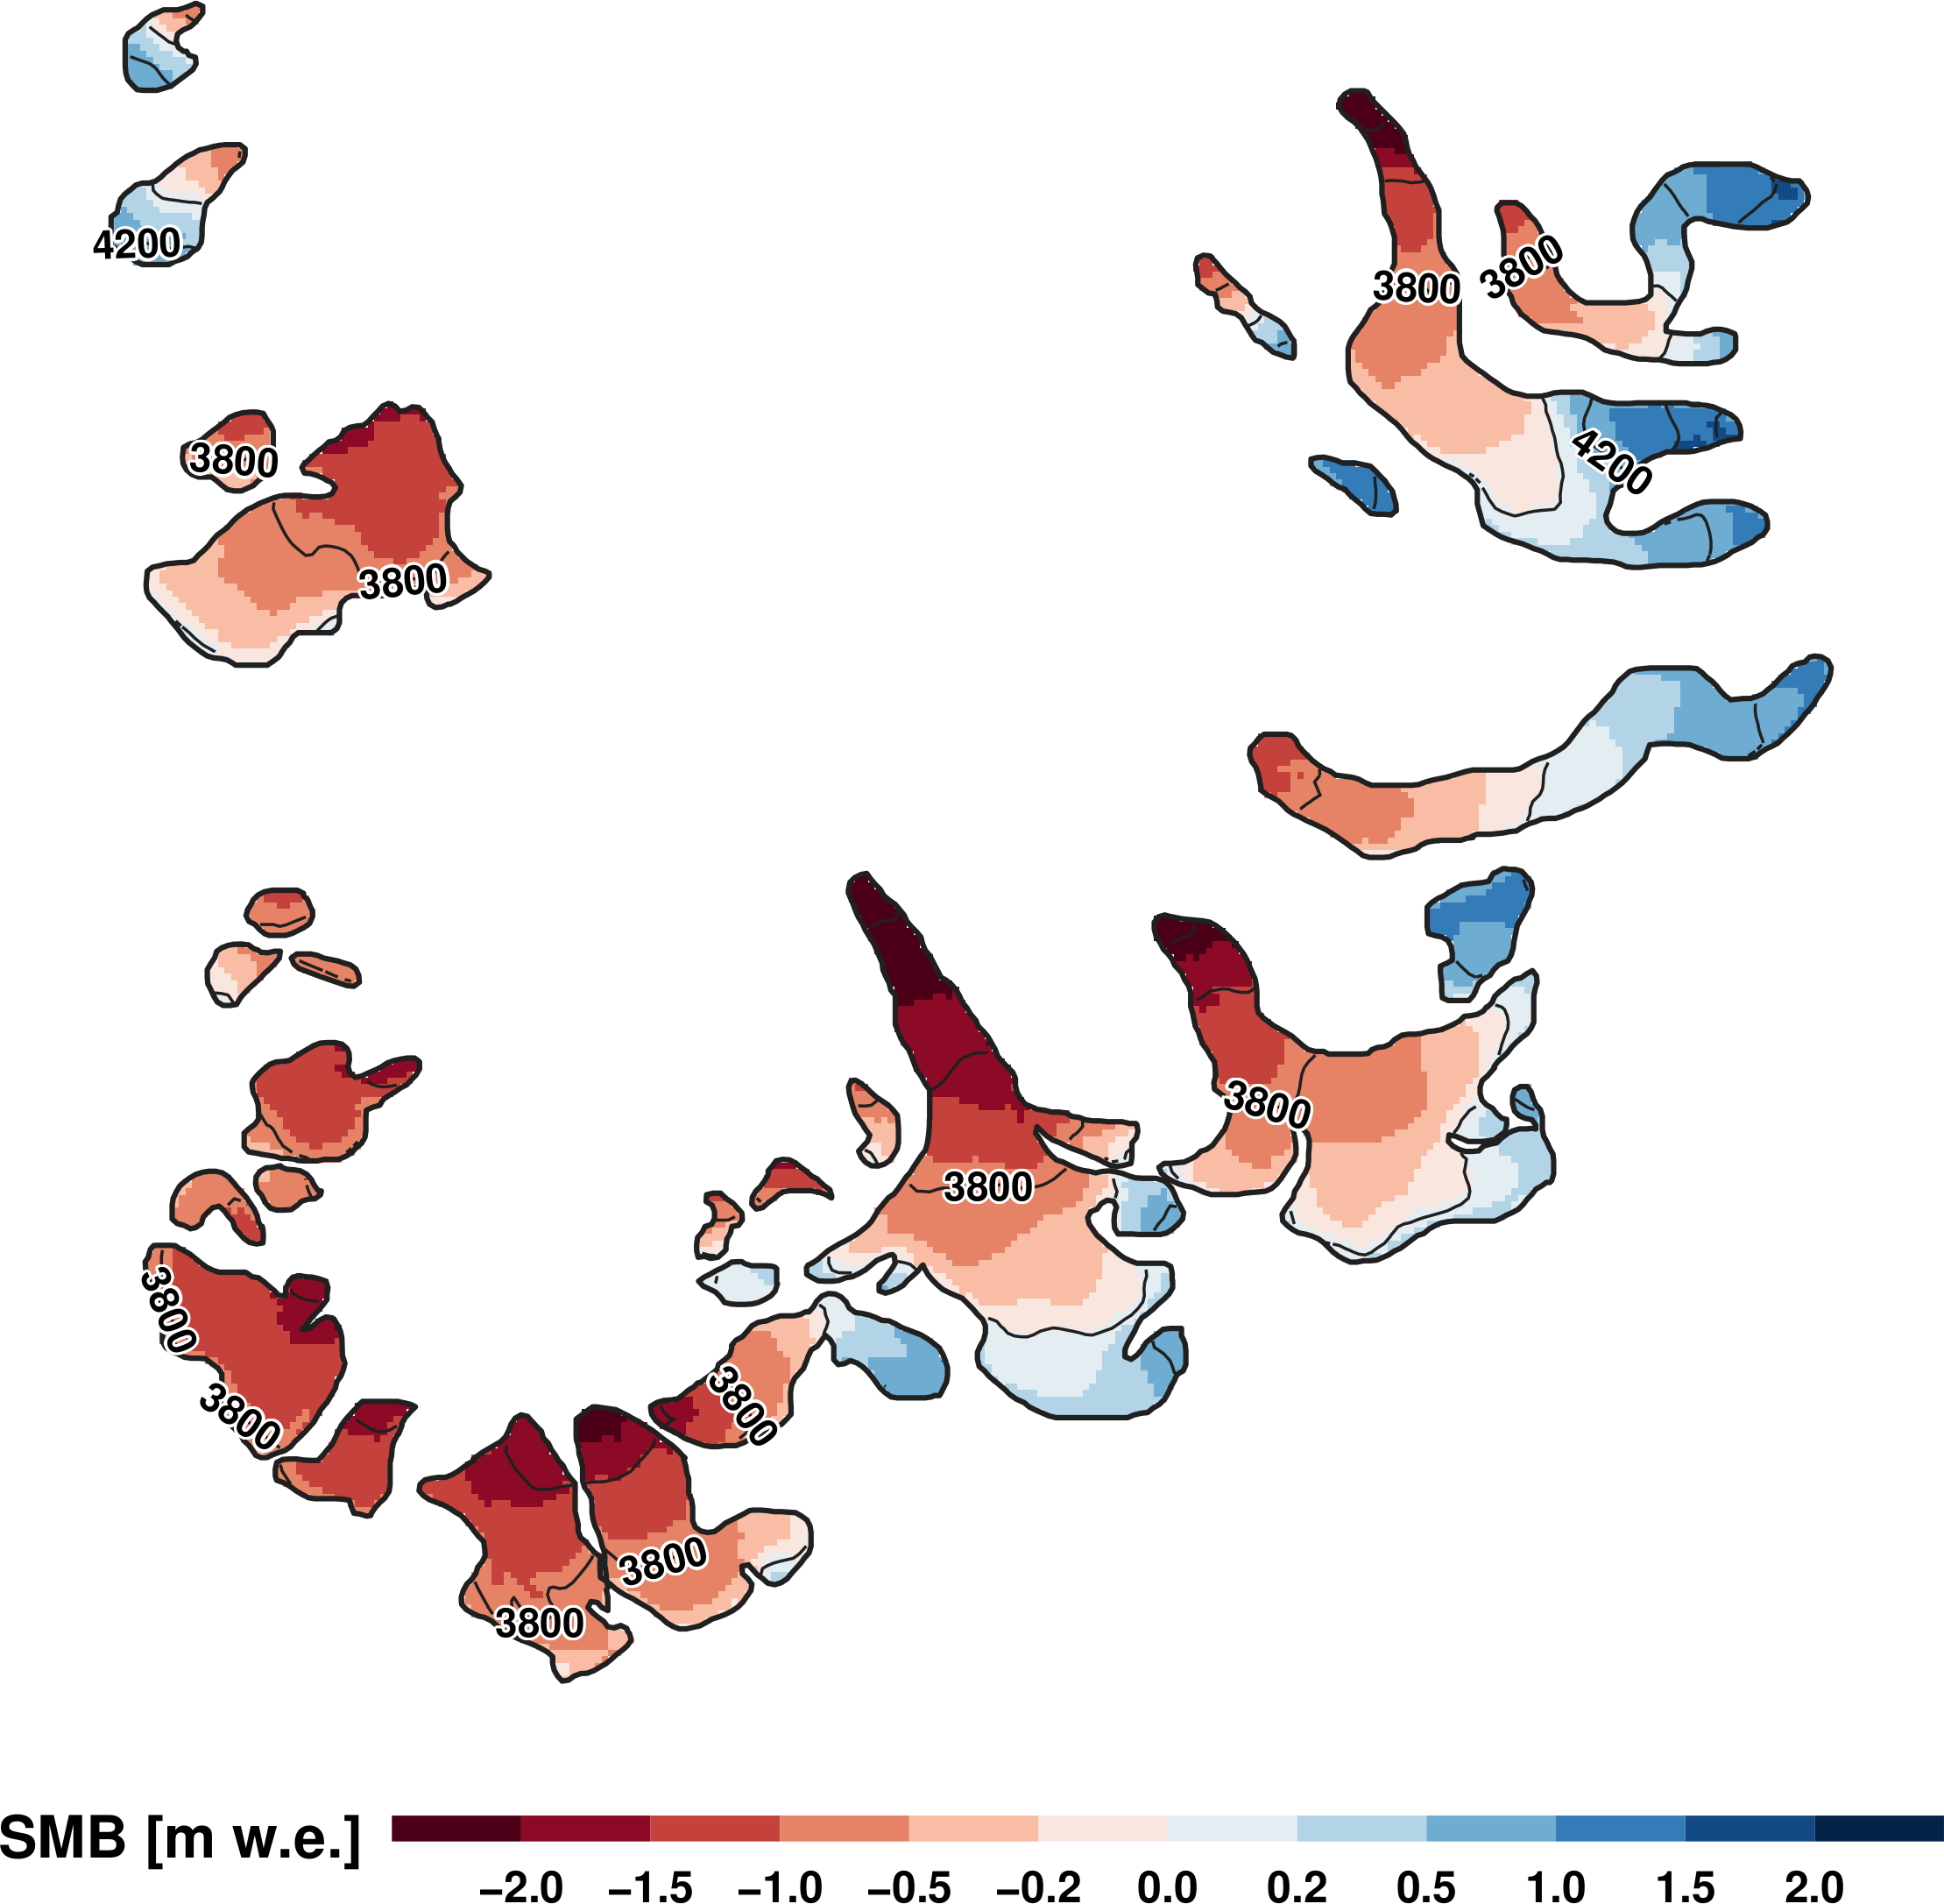
\includegraphics[width=12cm]{f0_cover_image}\par
	\vspace{1.3 cm}
	{\normalsize \textbf{Enrico Mattea}\\}
	{\normalsize \textit{enrico.mattea@unifr.ch\\}}
	\vspace{0.6 cm}
	{\normalsize October 2021}


	\vfill

\end{titlepage}


\section{Introduction}
In this second tutorial we are going to simulate the mass balance of Abramov glacier (Pamir Alay) from 1980 to 1994. Compared to the first tutorial, we will use some additional features of the model:

\begin{itemize}
    \item Multiple input files for different years
    \item Surface type with also firn and debris
    \item Advanced configuration with annual parameters
    \item Simulation of years with no measured mass balance
\end{itemize}
\textbf{Note:} to follow this tutorial you should be \textbf{already familiar with} the procedures of \textbf{tutorial 1.}

\clearpage
\section{Input files}
To prepare the input files we use the same methods explained in \textbf{section 3 of tutorial 1.} The input files will go in the model folder, under \textit{input\textbackslash abramov\textbackslash}.

\begin{itemize}
    \item The \textbf{meteo} and \textbf{mass balance} files are provided together with this tutorial, under \textit{tutorial2\_input\textbackslash abramov\textbackslash}. The mass balance file contains annual stake measurements from 1986/87 to 1989/90.
    \item On the \textbf{EarthExplorer} portal there is a good Landsat-5 image of the Abramov region taken on 22 August 1988, so we will create a \textbf{glacier outline shapefile} for the year 1988. The satellite image is located under \textbf{Data Sets $\rightarrow$ Landsat $\rightarrow$ Landsat Collection 2 Level-2 $\rightarrow$ Landsat 4-5 TM C2 L2}, and is called\\ LT05\_L2SP\_152033\_19880822\_20200917\_02\_T1. We download \textbf{band 3} ("...SR\_B3.TIF").
    \item In QGIS or ArcGIS we \textbf{draw the glacier outline} and we save it as a shapefile, called \textit{outline\_abramov\_1988.shp}.
    \item The model can use information on the \textbf{firn area} and the \textbf{debris cover} to make a better simulation of mass balance. On the satellite image of Abramov, we can see the late-summer snow line and the debris cover, so we can draw them:
    \begin{itemize}
        \item We make a copy of the glacier outline shapefile.
        \item We edit the glacier outline to \textbf{remove the glacier tongue,} leaving only the firn area. In QGIS, we can use the \textbf{Vertex Tool} to remove the glacier tongue (Fig. \ref{fig:f1_qgis_outl_firn_1988}).
        \item We save the new file as \textit{firn\_abramov\_1988.shp}.
        \item We make another copy of the outline shapefile.
        \item We edit the outline polygon to cover \textbf{only the debris} on the tongue.
        \item We save the new file as \textit{debris\_abramov\_1988.shp}.
        \item The three shapefiles are shown in Fig. \ref{fig:f2_qgis_all_files_1988}.
    \end{itemize}
    
\begin{figure}[htp!]
    \centering
    \includegraphics[width=1.0\textwidth]{f1_qgis_outl_firn_1988}
    \caption{Editing the glacier outline to create the firn shapefile in QGIS.}
    \label{fig:f1_qgis_outl_firn_1988}
\end{figure}

\begin{figure}[hbp!]
    \centering
    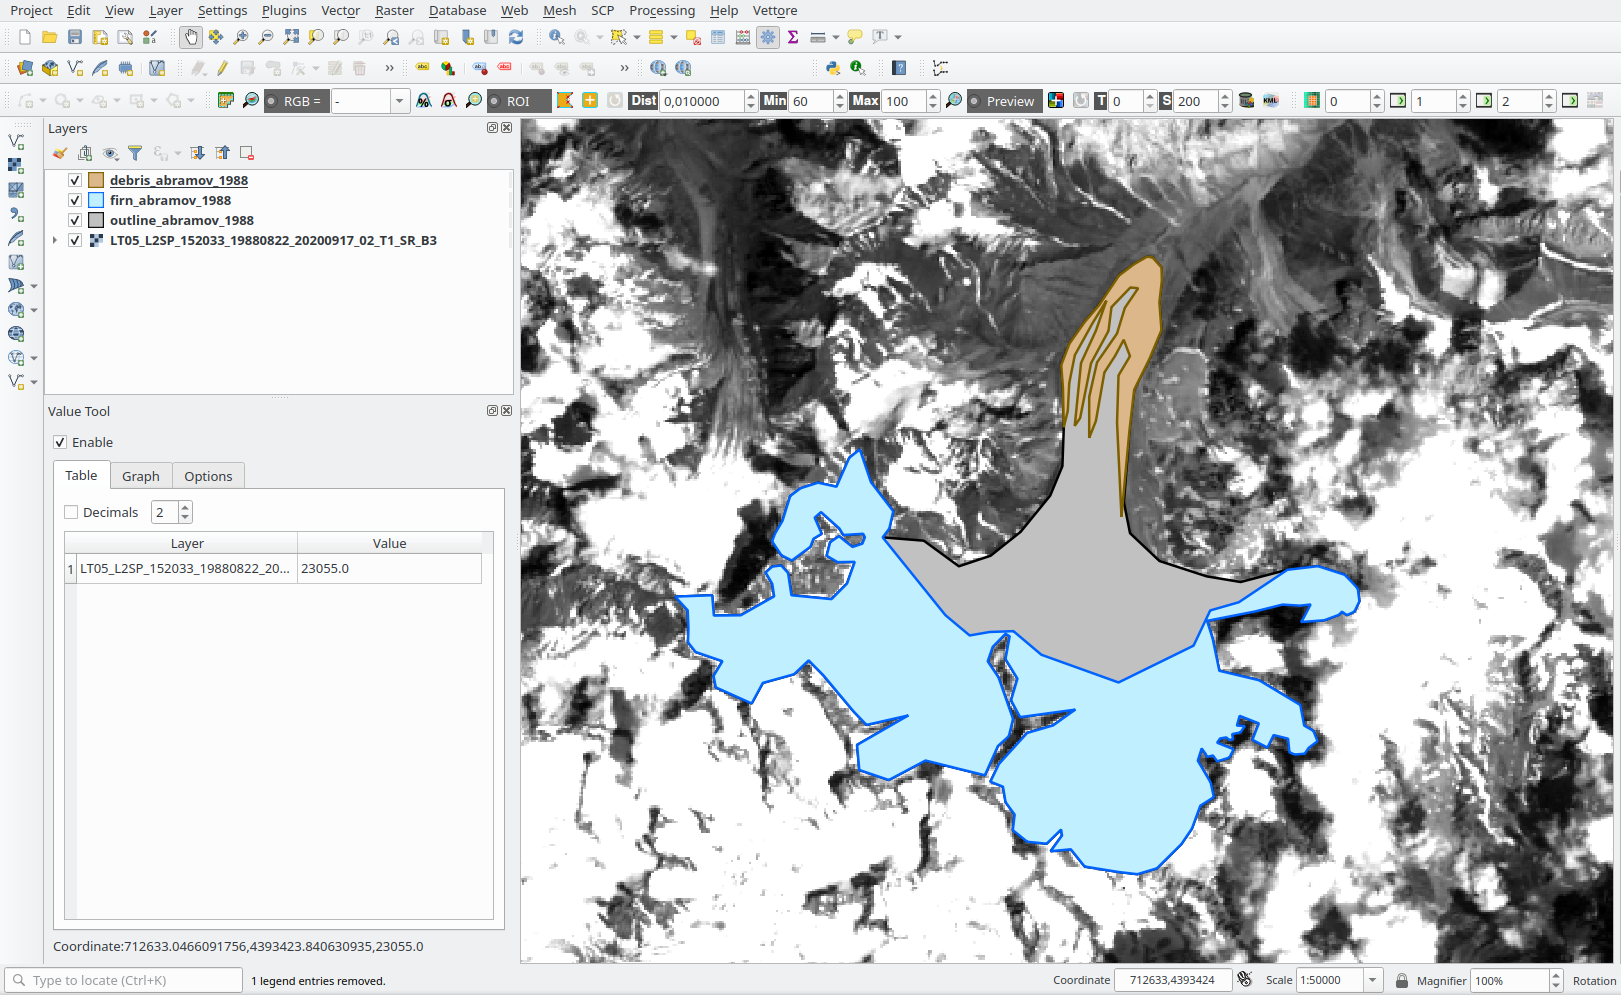
\includegraphics[width=1.0\textwidth]{f2_qgis_all_files_1988}
    \caption{The outline (grey), firn (blue) and debris (yellow) shapefiles at Abramov for year 1988.}
    \label{fig:f2_qgis_all_files_1988}
\end{figure}
 
    \item The glacier area changes over time (retreat of the tongue). The model can use \textbf{different outline files} (up to one per each year) to follow these glacier changes. We create a \textbf{second outline shapefile} corresponding to year 1994:
    \begin{itemize}
        \item From the EarthExplorer we download image LT05\_L2SP\_152032\_19940823\_20200913\_02\_T1 (band 3, from 23 August 1994) and we load it into QGIS or ArcGIS.
         \item To create the outline, we can \textbf{simply modify the 1988 outline.} We start by making a copy of \textit{outline\_abramov\_1988.shp}.
         \item We \textbf{adjust the tongue} (Vertex Tool, as in Fig. \ref{fig:f1_qgis_outl_firn_1988}) so that it covers the 1994 extent (Fig. \ref{fig:f3_qgis_outl_1988_1994}).
         \item We save the shapefile as \textit{outline\_abramov\_1994.shp}.
         \item On the image there is \textbf{not a big change of firn and debris,} so we don't make new shapefiles for firn or debris: we will \textbf{re-use the shapefiles from 1988.}
    \end{itemize}

\begin{figure}[ht]
    \centering
    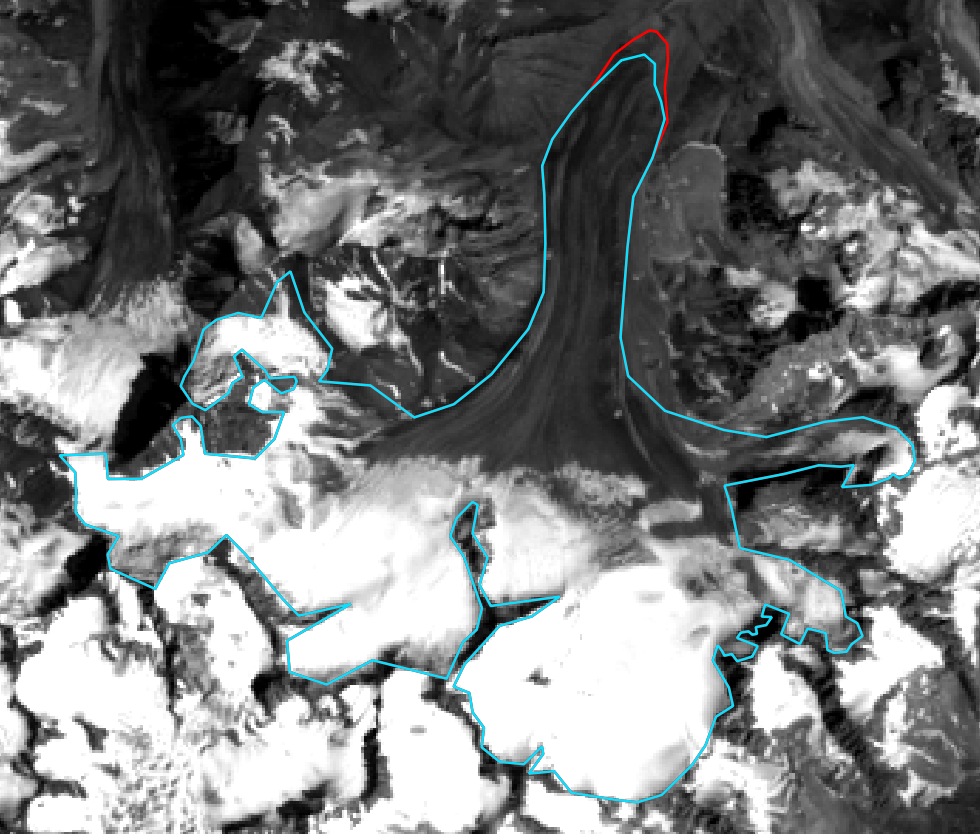
\includegraphics[width=0.6\textwidth]{f3_qgis_outl_1988_1994}
    \caption{The 1988 (red) and 1994 (blue) outlines of Abramov glacier. Note that most of the 1988 outline is covered by the 1994 one.}
    \label{fig:f3_qgis_outl_1988_1994}
\end{figure}

    \item For the \textbf{DEM}, we download the ASTER file ASTGTMV003\_N39E071 (GeoTiff format).
    
    \item As in the first tutorial, we open program \textit{make\_input.R} with RStudio and we click on \textbf{Run App}.
    
    \item First we make the input for year 1988:
    \begin{itemize}
        \item \textbf{glacier name} \textit{abramov}
        \item\textbf{model year} 1988
        \item \textbf{DEM file} \textit{ASTGTMV003\_N39E071\_dem.tif}
        \item \textbf{glacier shapefile} \textit{outline\_abramov\_1988.shp}
        \item \textbf{firn shapefile} \textit{firn\_abramov\_1988.shp}
        \item \textbf{debris shapefile} \textit{debris\_abramov\_1988.shp}
        \item \textbf{margin size} 500 m
        \item \textbf{grid cell size} 50 m
        \item Check \textbf{compute radiation.}
    \end{itemize}
    
    \item We click on \textbf{RUN}
    \item When the processing is finished, we close the \textit{make\_input} window and we click again on \textbf{Run App} to make the input for year 1994.
    
    \item For year 1994 we use the following input:
        \begin{itemize}
        \item \textbf{glacier name} \textit{abramov}
        \item\textbf{model year} 1994
        \item \textbf{DEM file} \textit{ASTGTMV003\_N39E071\_dem.tif}
        \item \textbf{glacier shapefile} \textit{outline\_abramov\_\textbf{1994}.shp}
        \item \textbf{firn shapefile} \textit{firn\_abramov\_1988.shp}: as said before, \textbf{we use again the same firn} of 1988
        \item \textbf{debris shapefile} \textit{debris\_abramov\_1988.shp}: as said before, we use again the \textbf{same debris} of 1988
        \item \textbf{NOTE:} for the first time, we also use the \textbf{reference grid file} button. We select the file located under \textit{utils\textbackslash abramov\textbackslash dhm\textbackslash dhm\_abramov\_1988.tif}. The \textbf{reference grid file} is used to \textbf{align} the 1994 files \textbf{to the same area} of 1988. The model can also work without this, but it will be \textbf{faster and more accurate} if we use it
        \item \textbf{margin size} 500 m
        \item \textbf{grid cell size} 50 m
        \item Don't check \textbf{compute radiation}: we use again the \textbf{same radiation} of 1988.
    \end{itemize}
    \item When \textit{make\_input} has finished, we move the \textit{utils\textbackslash abramov\textbackslash} folder to the model folder, under \textit{input\textbackslash}.
    \item The input folder (\textit{input\textbackslash abramov\textbackslash}) looks like Fig. \ref{fig:f4_input_folder}.
\end{itemize}

\begin{figure}[hb!]
    \centering
    \includegraphics[width=0.7\textwidth]{f4_input_folder}
    \caption{The folder \textit{input\textbackslash abramov\textbackslash} after preparing all the input data.}
    \label{fig:f4_input_folder}
\end{figure}


\clearpage
\section{Model parameters}

As usual, parameters are set in file \textit{set\_params.R}. We set the main parameters as in Table \ref{table:t1_main_parameters}:

\begin{table}[h!]
\caption{main model parameters.}
\label{table:t1_main_parameters}
\centering
\begin{tabularx}{\textwidth}{|l l X|} 
 \hline
 \textbf{Parameter name} & \textbf{Value} & \textbf{Explanation} \\ [0.5ex] 
 \hline
 name\_glacier & "abramov" & Glacier name \\ 
 \hline
 filename\_weather & "weather\_abramov.dat" & Name of the meteo file \\
 \hline
 file\_weather\_nskip & 2 & Number of lines to skip in the meteo file \\
 \hline
 grids\_crs & 32642 & EPSG code of the coordinates system \\
 \hline
 filename\_massbalance\_annual & "mb\_abramov.dat" & Name of the file with the annual mass balance measurements\\
 \hline
 filename\_massbalance\_winter & "" & Name of the file with the winter mass balance measurements. We don't have this so we leave it empty ("")\\
 \hline
 weather\_aws\_elevation & 3837 & Altitude of the meteo data.\\
 \hline
 first\_year & 1980 & First year that we want to simulate: 2020\\
 \hline
 last\_year & 1994 & Last year that we want to simulate\\
 \hline
\end{tabularx}
\end{table}

Compared to tutorial 1 we set \textbf{some additional parameters} (Table \ref{table:t2_additional_parameters}):


\begin{table}[h!]
\caption{additional model parameters for the Abramov multi-year simulation.}
\label{table:t2_additional_parameters}
\centering
\begin{tabularx}{\textwidth}{|l l X|} 
 \hline
 \textbf{Parameter name} & \textbf{Value} & \textbf{Explanation} \\ [0.5ex] 
 \hline
 weather\_max\_precip\_ele & 4600 & On a glacier, \textbf{precipitation} usually \textbf{increases} with altitude, but \textbf{only up to a certain limit,} above which it decreases. This parameter defines that limit (in meters a.s.l.)\\
 \hline
 model\_avalanche\_dates & c("3/31", "6/30") & This parameter defines the \textbf{dates at which an avalanche is simulated,} as "month/day". The avalanche redistributes snow at the base of steep slopes. \textbf{Note the \textit{c}} at the beginning, which is used to combine the values. To remove avalanches completely, we would simply use c().\\
 \hline
 debris\_red\_fac & 0.9 & This parameter defines the \textbf{reduction of melt} for glacier cells which are covered by debris (supraglacial \textbf{moraine}). 1 = no reduction, 0.5 = melt is reduced by half.\\ 
 \hline
 default\_prec\_corr & 300 & Precipitation measured at a meteo station is usually underestimated \textbf{(precipitation undercatch)}. This parameter defines a \textbf{precipitation correction} in percent (100 = no correction, 200 = double the precipitation).\\
 \hline
 default\_prec\_summer\_fact & 0.7 & Precipitation undercatch at a meteo station can be a bigger problem in winter than in summer. This parameter \textbf{reduces the previous precipitation correction} from May to September (1 = no reduction, 0.5 = reduction by half)\\
 \hline
 nodata\_years\_automatic & TRUE & This parameter tells the model \textbf{what to do with the years which have no mass balance measurements.} TRUE = use the mean optimized parameters from the years which have data, FALSE = use the values from \textit{set\_params.R} (like default\_melt\_factor).\\
 \hline
 
\end{tabularx}
\end{table}

\clearpage
\section{Running the model}
We run the model as in tutorial 1, by opening file \textit{main.R} in RStudio and clicking on \textit{Source}. The model output is stored under \textit{output\textbackslash abramov\textbackslash}. After the model has finished, we can see a \textbf{summary of the simulation results} under \textit{output\textbackslash abramov\textbackslash overview.pdf}. Figure \ref{fig:f5_melt_parameters} (from \textit{overview.pdf}) shows the model parameters optimized for each year. Note how the years with no data have a constant value which corresponds to the mean of the other years: this is the effect of parameter nodata\_years\_automatic (Table \ref{table:t2_additional_parameters}). Figure \ref{fig:f6_cumulative_mb} shows the cumulative annual mass balance over the modeled period. The years with no data have a dashed line. 



\begin{figure}[ht]
    \centering
    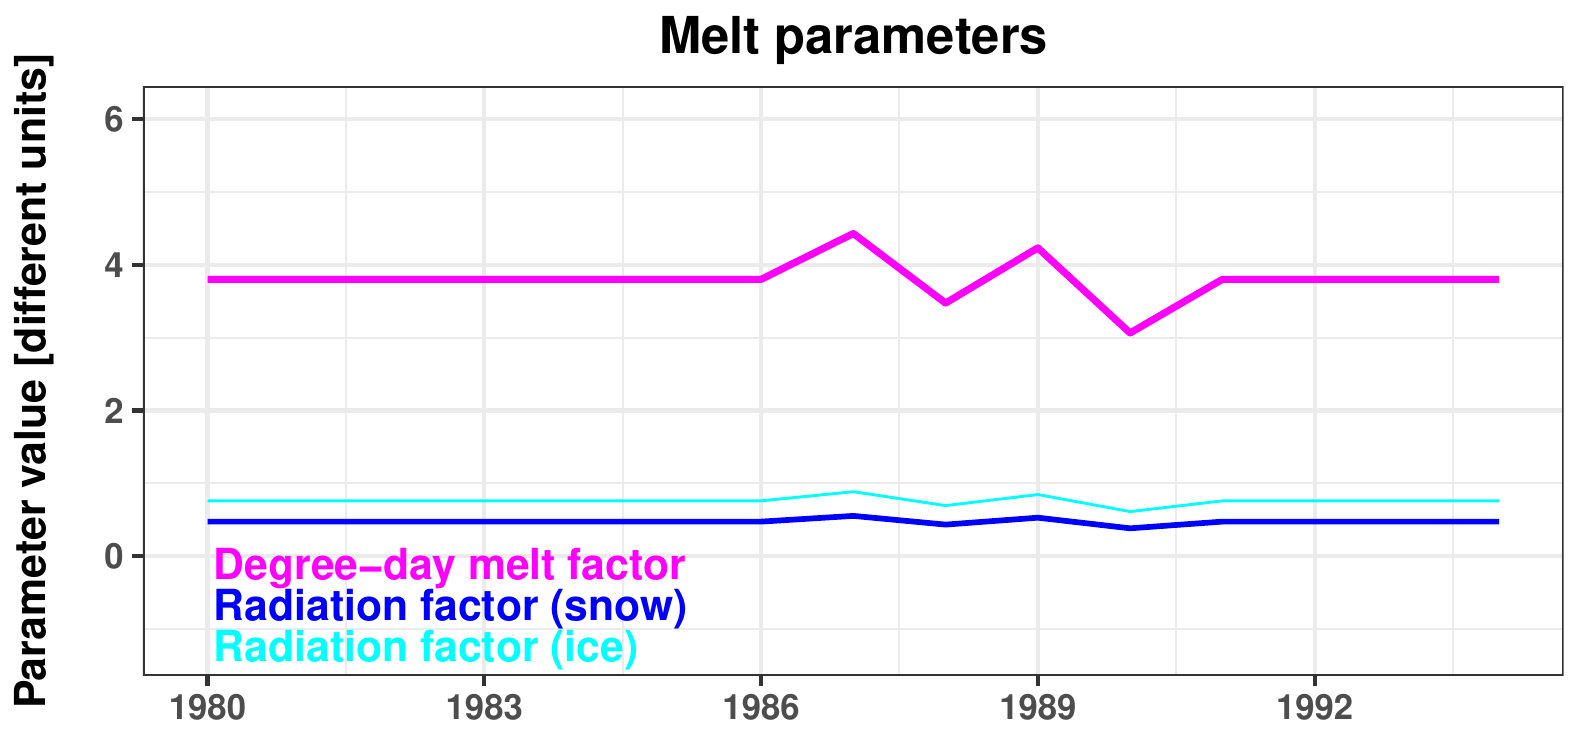
\includegraphics[width=0.9\textwidth]{f5_melt_parameters}
    \caption{optimized model parameters for the multi-year simulation.}
    \label{fig:f5_melt_parameters}
\end{figure}

\begin{figure}[ht]
    \centering
    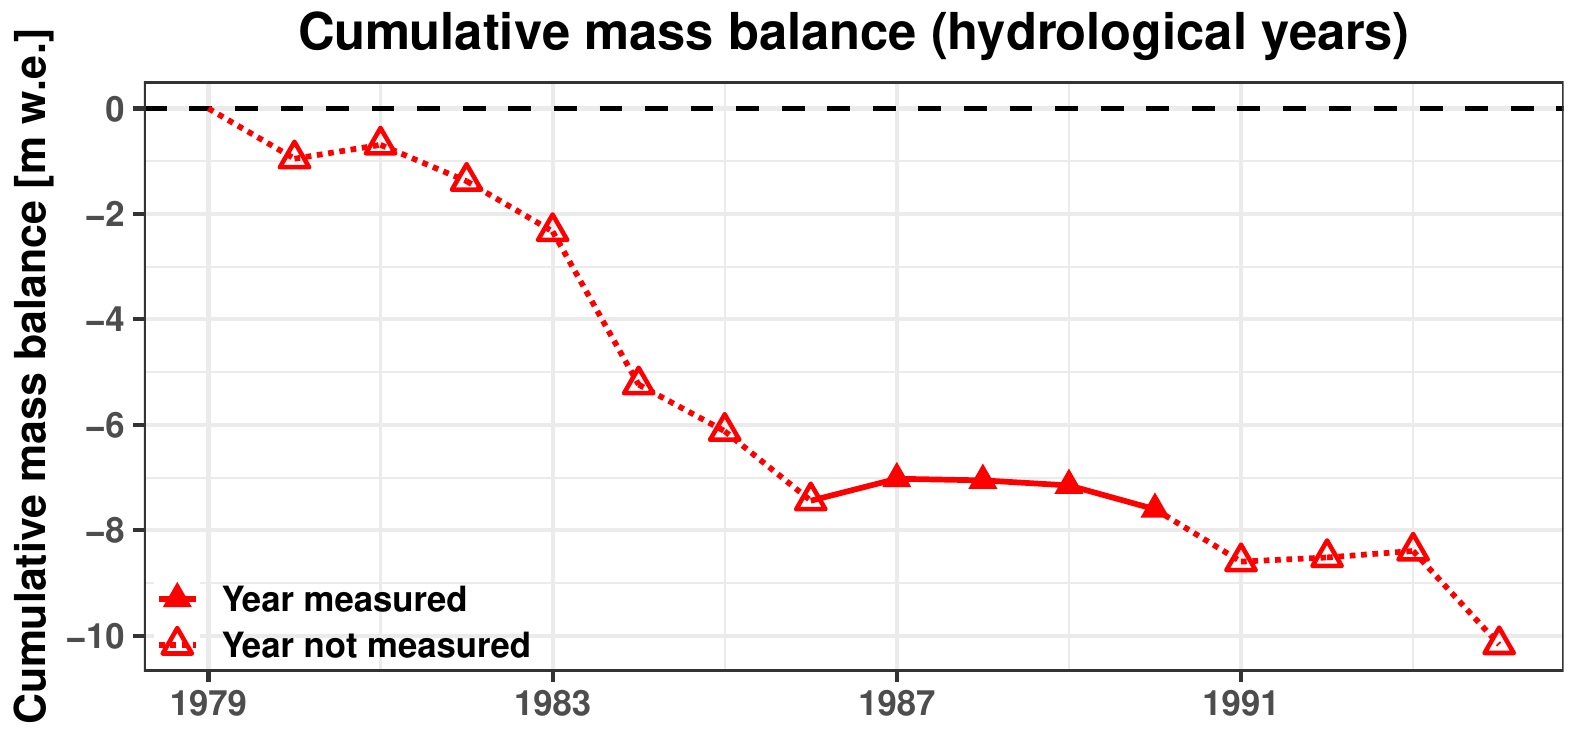
\includegraphics[width=0.9\textwidth]{f6_cumulative_mb}
    \caption{cumulative annual mass balance over the modeled period.}
    \label{fig:f6_cumulative_mb}
\end{figure}


\clearpage
\section{Improving the simulation}
\noindent The plot of the simulated RMS errors (Fig. \ref{fig:f7_rms}) shows that in the years 1987/88 and 1989/90 the model performed less well than the other years (RMS is higher). If we look at the \textbf{detailed annual results} (Fig. \ref{fig:f8_mb_profile_before}, in \textit{output\textbackslash abramov\textbackslash annual\_results\textbackslash}), we can see that \textbf{the error depends on the altitude:} the modeled mass balance is too low near the glacier source, and too high on the glacier tongue. We can improve the simulation by \textbf{changing some parameters for these years only.}
To change these annual parameters, we create a new folder under \textit{input\textbackslash abramov\textbackslash}, called \textit{params\textbackslash}. Inside we put a new file called \textit{param\_1988.dat}, with the content shown in Fig. \ref{fig:f9_param_file}. In this example, we change both the precipitation correction and the gradient of precipitation with altitude. In general, the parameter file can change any of the parameters of Table \ref{table:t3_param_file}. If the model finds a \textbf{parameter file} for a certain year, these values are used \textbf{instead of} the ones from \textbf{\textit{set\_params.R.}} An example of a full parameter file is shown in Fig. \ref{fig:f10_param_file_full}. In the parameter file all lines starting with an asterisk (*) are ignored. For 1989/90, we use just one annual parameter: prec\_corr = 310. We put it in a file called \textit{param\_1990.dat}. Then \textbf{we run the model again} and we see that the simulation is improved (lower RMS for these years).


\begin{table}[h!]
\caption{parameters which can be set for a specific year in the annual parameters file (also see Table \ref{table:t2_additional_parameters}).}
\label{table:t3_param_file}
\centering
\begin{tabularx}{\textwidth}{|l l X|} 
 \hline
 \textbf{Parameter name} & \textbf{Unit} & \textbf{Explanation} \\ [0.5ex] 
 \hline
 prec\_corr & \% & Precipitation correction\\
 \hline
 prec\_elegrad & \% / 100 m & Gradient of precipitation with altitude\\
 \hline
 prec\_summer\_fact & - & Reduction of precipitation correction in summer\\
 \hline
 temp\_elegrad & \degree C / 100 m & Gradient of air temperature with altitude\\
 \hline
 melt\_factor & mm w.e. / (\degree C day) & Melt factor for temperature\\
 \hline
 rad\_fact\_ice & 10\textsuperscript{-3} mm w.e. / (\degree C hour (W m\textsuperscript{-2})) & Ice melt factor for solar radiation\\
 \hline
 rad\_fact\_snow & 10\textsuperscript{-3} mm w.e. / (\degree C hour (W m\textsuperscript{-2})) & Snow melt factor for solar radiation\\
 \hline
 
\end{tabularx}
\end{table}




\begin{figure}[ht]
    \centering
    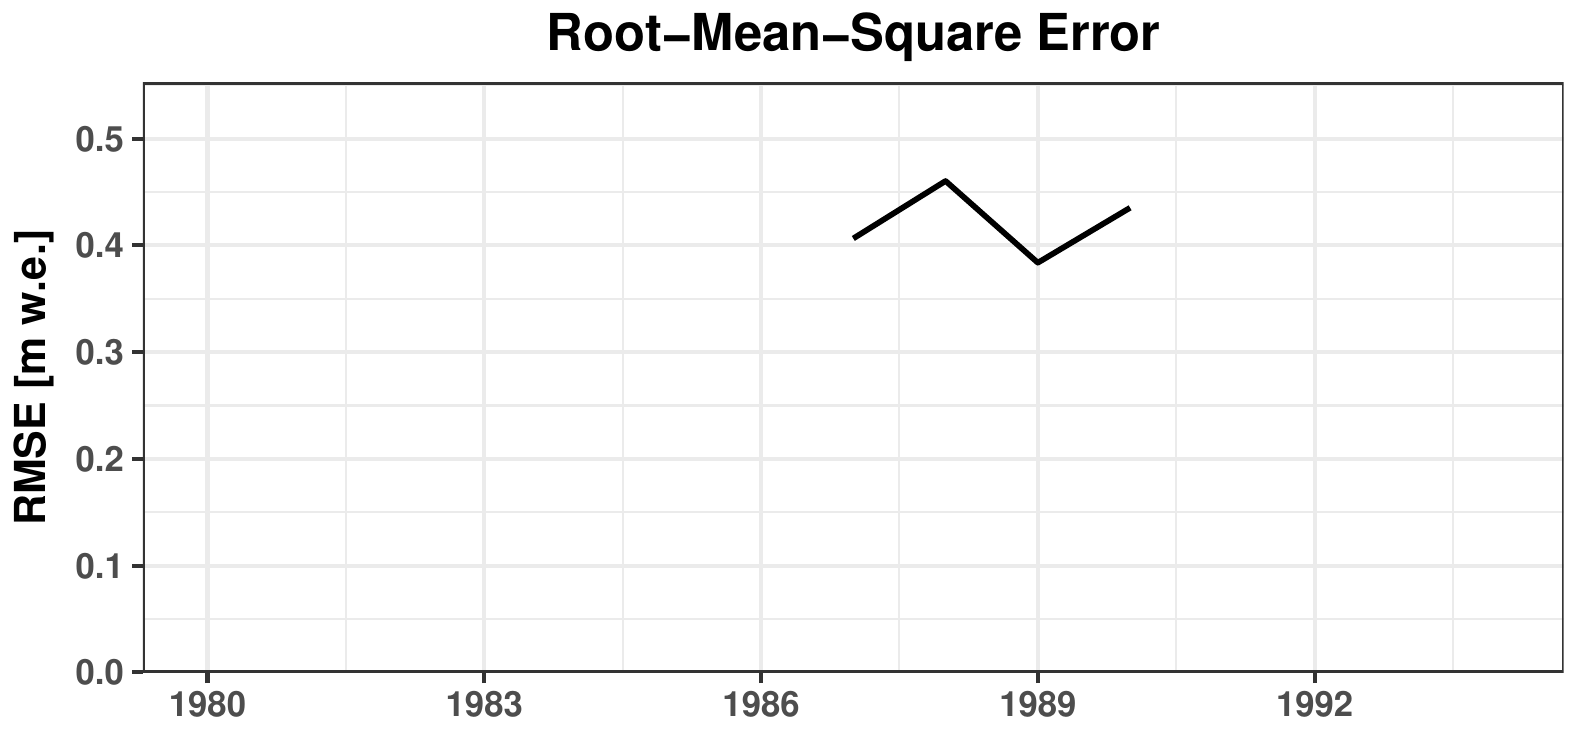
\includegraphics[width=0.9\textwidth]{f7_rms}
    \caption{RMS error for the multi-year simulation.}
    \label{fig:f7_rms}
\end{figure}

\begin{figure}[ht]
    \centering
    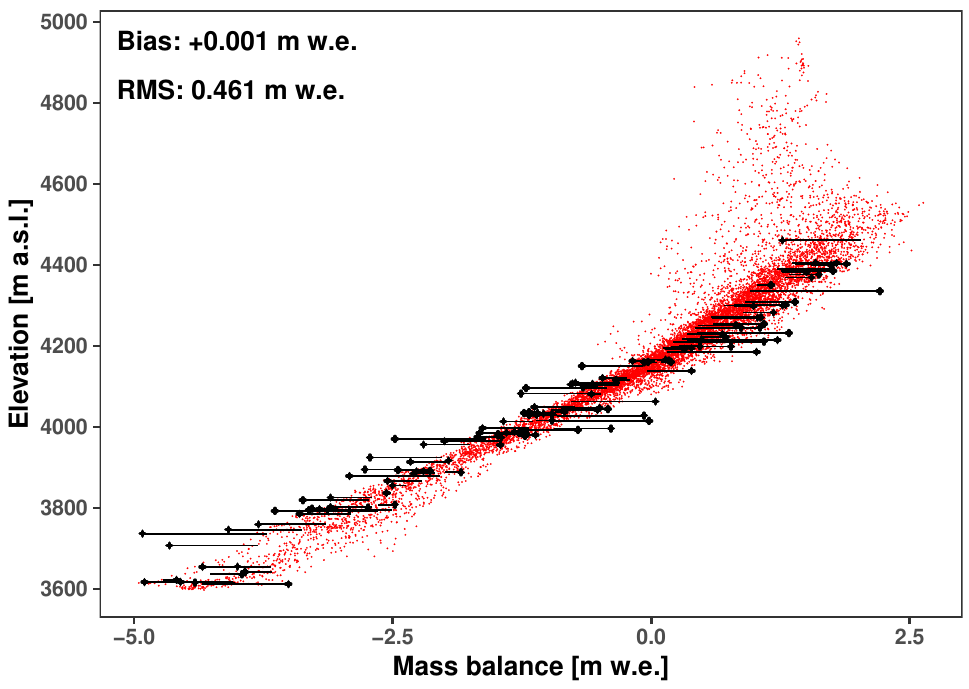
\includegraphics[width=0.9\textwidth]{f8_mb_profile_before}
    \caption{modeled mass balance profile (red) and stake measurements (black) for year 1987/1988.}
    \label{fig:f8_mb_profile_before}
\end{figure}

\begin{figure}[ht]
    \centering
    \includegraphics[width=0.9\textwidth]{f9_param_file}
    \caption{parameter file for year 1988.}
    \label{fig:f9_param_file}
\end{figure}

\begin{figure}[ht]
    \centering
    \includegraphics[width=0.9\textwidth]{f10_param_file_full}
    \caption{example parameter file with all the parameters which can be set.}
    \label{fig:f10_param_file_full}
\end{figure}


\end{document}
